% id: 59-11
% book: 베이직쎈 확률과 통계 · 03 확률의 뜻과 활용
% section: 실전 감각 UP
% figure: tikz:fig-59-11
% answer: 
% answer_source: 
% variant_level: 0 (원본 전사)
% 이 파일은 build.mjs 가 items.json 에서 만든다. 고칠 때는 items.json 을 고친다.
\smash{\raisebox{1.5mm}{\dmkichul{베이직쎈 확률과 통계 59쪽 11번}}}
\noindent\begin{minipage}[t]{0.58\linewidth}\vspace{0pt}\raggedright 오른쪽 그림과 같은 도로망이 있다. $\pt{P}$에서 $\pt{Q}$까지 최단 거리로 갈 때, $\pt{A}$를 거치지 않을 확률은? \dmcondfill{각 경로를 택할 확률은 같은 것으로 생각한다.}{}\end{minipage}\hfill\begin{minipage}[t]{0.4\linewidth}\vspace{0pt}\centering \resizebox{\ifdim\width>\linewidth\linewidth\else\width\fi}{!}{% 59-11(인쇄 59쪽) — 가로 4칸·세로 3칸 도로망. P 는 왼쪽 아래 모퉁이, Q 는 오른쪽 위 모퉁이, A 는 P 에서 오른쪽 1칸·위 1칸인 교차점.
% 스캔 그림이 흐려 TikZ 로 다시 그림. 라벨은 원문에 있는 P·Q·A 셋뿐이고 경로 수는 적지 않는다.
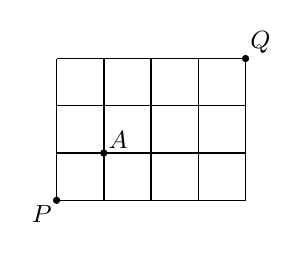
\begin{tikzpicture}[scale=0.6, line width=0.5pt]
  \draw[step=1] (0,0) grid (4,3);
  \fill (0,0) circle (2.2pt);
  \fill (4,3) circle (2.2pt);
  \fill (1,1) circle (2.2pt);
  \node[anchor=north east, inner sep=1.5pt, font=\small] at (0,0) {$\pt{P}$};
  \node[anchor=south west, inner sep=1.5pt, font=\small] at (4,3) {$\pt{Q}$};
  \node[anchor=south west, inner sep=1.5pt, font=\small] at (1,1) {$\pt{A}$};
\end{tikzpicture}
}\end{minipage}\par
\dmchoicesauto{\rule[-3ex]{0pt}{8ex}}{$\dfrac{3}{14}$}{$\dfrac{2}{7}$}{$\dfrac{5}{14}$}{$\dfrac{3}{7}$}{$\dfrac{1}{2}$}
